\subsection{Эксперимент 5. Векторизация текстов. Выбор параметров min\_df и max\_df}
\subsubsection{Дизайн эксперимента}
Заданы: \\
\begin{itemize}
	\item Общие значения параметров, по которым идет перебор:
	\begin{enumerate}
		\item $min\_df = 0.00001, 0.0001, 0.01, 0.1, 0.3$
		\item  $max\_df = 0.1, 0.25, 0.35, 0.45, 0.55, 0.7$
	\end{enumerate}
	\item Для GD:
	\begin{enumerate}
		\item $\alpha = 0.1$
		\item  $\beta = 0.01$
		\item  $\omega_0 = 0 \in \mathbb{R}^D$
	\end{enumerate}
	\item Для SGD:
	\begin{enumerate}
		\item $\alpha = 0.1$
		\item  $\beta = 0.0347$
		\item  $\omega_0 = 0 \in \mathbb{R}^D$
		\item  $batch\_size = 10000 $
	\end{enumerate}
\end{itemize}

В данном эксперименте анализируется влияние на точность, время работы, размер признакового пространства различных методов векторизации текстов, параметров min\_df и  max\_df. В качестве методов векторизации будут рассмотрены два метода:
{\bf BagOfWords(BOW)}, основанный на подсчете количества повторений уникальных слов, и {\bf Tf-Idf}, основанный на подсчете количества повторений уникальных слов с поправкой на частоту встречаемости во всей коллекции текстов. После изучения векторизации, будет рассмотрен min\_df, а уже после того, как будет найден оптимальный min\_df будет изучен вопрос об оптимальном max\_df. Также стоит отметит, что в ходе этого эксперимента в качестве валидационной и обучающей выборки брались валидационноая и обучающую выборка, которая обсуждалась в самом начале раздела "Список экспериментов".
\subsubsection{Результаты эксперимента}
\begin{enumerate}
	\item {\bf BagOfWords и Tf-Idf}\\ \\
	\begin{tabular}{|c|c|c|c|c|}
		\hline
			Метод & Вид векторизации & Время (с)  & Количество признаков & $accuracy$ \\
		\hline
		\hline
			GD 
			& BOW & 7.759336 &  16050 &  0.806100\\ \cline{2-5}
			& Tf-Idf & 6.127796 & 16050 & 0.721500 \\
		\hline
			SGD 
			& BOW & 11.931548 &  16050 & 0.814100 \\ \cline{2-5}
			& Tf-Idf & 8.624678 & 16050 & 0.723900 \\
		\hline
	\end{tabular}\\

	Таблица выше была построена по предсказаниям на валидационной выборке.Заметим, что при данных методах векторизации размерность признакового пространства не изменяется. Время незначительно, но все же меньше в обоих случаях при использовании Tf-Idf. Что же касается $accuracy$, то, вероятно, в текстах часто можно встретить слова, например, "you"{}, "like"{}, которые, вообще говоря, присутствуют во многих текстах, а значит, будут иметь маленький вес в Tf-Idf. При этом количество этих слов сильно возрастает в токсичных текстах для сравнения человека с чем-то, поэтому хотелось бы, чтобы мы это как-то учитывали в модели, но из-за малых весов эта информация не будет почти учитываться. \\
	{\bfseriesПримеры: }
	\begin{itemize}
		\item "fuck you  you stupid american"
		\item "you are such a dickhead  you lesbian butch"
	\end{itemize}
	
	\item {\bf min\_df}\\ 
	
	\begin{figure*}[h]
        \begin{subfigure}{.5\textwidth}
            \centering
            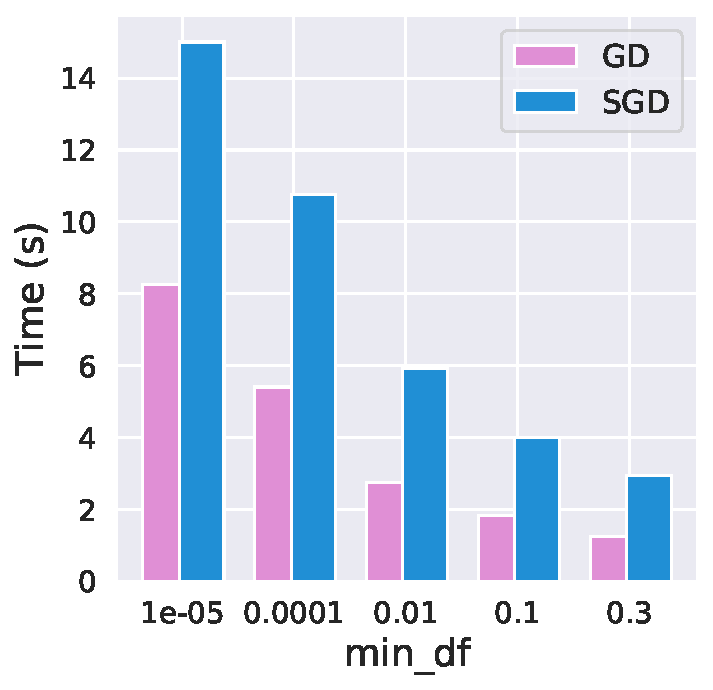
\includegraphics[width=0.9\linewidth]{./experiment5/mindf_time.pdf}
            \caption{}
        \end{subfigure}%
        \begin{subfigure}{.5\textwidth}
            \centering
            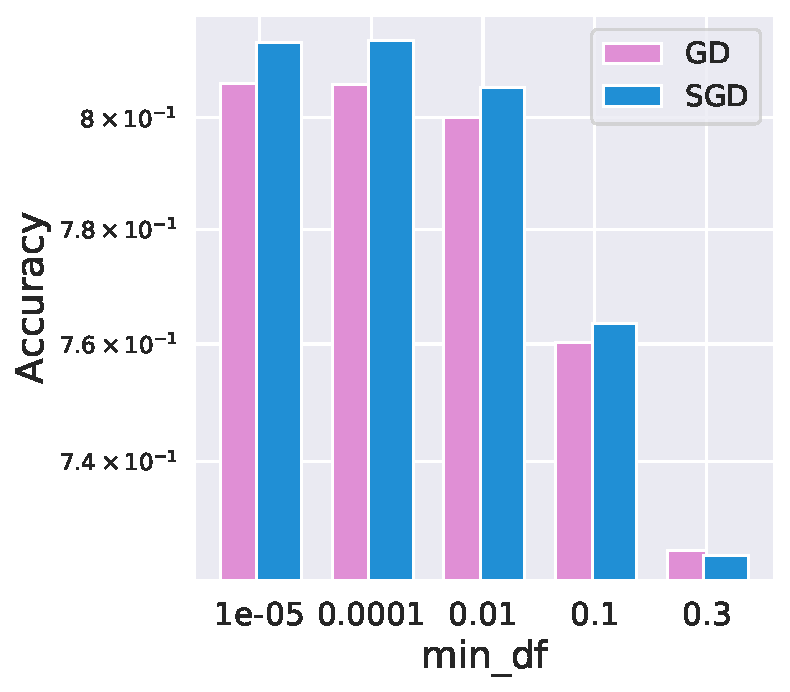
\includegraphics[width=\linewidth]{./experiment5/mindf_acc.pdf}
            \caption{}
        \end{subfigure}
    \caption{}\label{eq:exp5_fig1}
    \end{figure*}
	Из рис.\ref{eq:exp5_fig1} видно, что чем меньше  значение 
	$min\_df$, тем GD и SGD больше тратят времени на минимизацию функционала $Q(w)$, это неудивительно, так как размер признакового пространства увеличивается (см. таблицу ниже)\footnote{Оценки вычислительной сложности GD и SGD были даны выше в эксперименте 3}. Также из графика зависимости $accuracy$ от $min\_df$ видно, что при $min\_df\lessapprox 0.0001$ точность примерно такая же как и при $min\_df =0.0001$ (при $min\_df = 0.0001$ она даже выше чем при $min\_df =10^{-5}$ : 0.8141 против 0.8137), а при $min\_df \gtrapprox 0.0001$ уже начинается падение точности. Видимо, при больших $min\_df$ слишком много полезных признаков пропадает, так как признак(слово) выкидывается тогда, когда частота его встречаемости во всех текстах меньше заданного значения $min\_df$.

	\item {\bf max\_df}\\ 
	
	Фиксируем теперь оптимальный $min\_df = 0.0001$. Тут со временем ситуация такая же как и у $min\_df$ с увеличением $max\_df$ увеличивается признаковое пространство (см. таблицу ниже и рис.\ref{eq:exp5_fig3}), поэтому и время увеличивается. 
	\begin{figure*}[h]
        \begin{subfigure}{.5\textwidth}
            \centering
            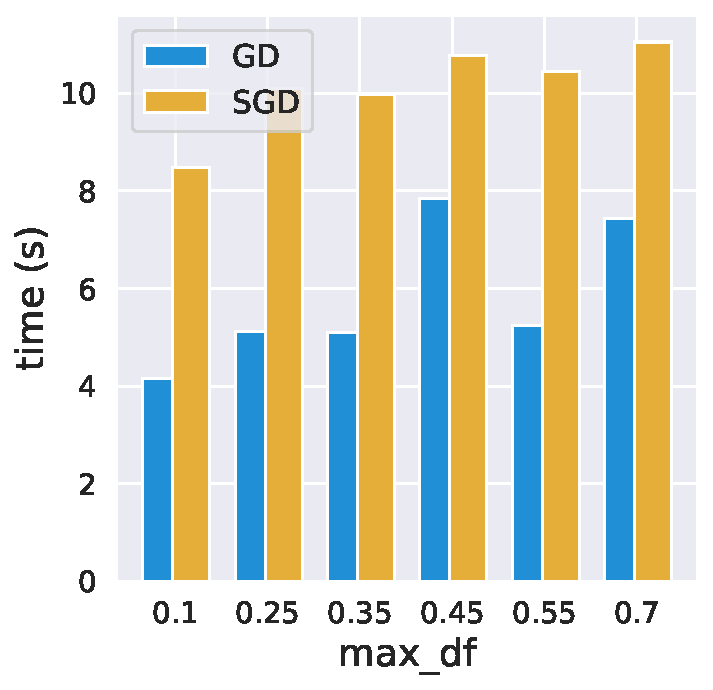
\includegraphics[width=0.9\linewidth]{./experiment5/maxdf_time.pdf}
            \caption{}
        \end{subfigure}
        \begin{subfigure}{.5\textwidth}
            \centering
            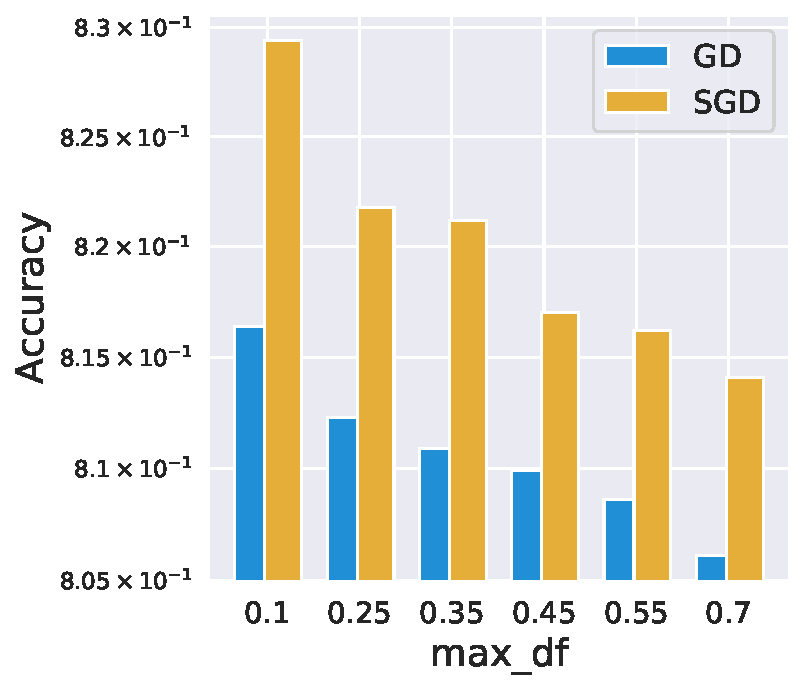
\includegraphics[width=\linewidth]{./experiment5/maxdf_acc.pdf}
            \caption{}
        \end{subfigure}
    \caption{}\label{eq:exp5_fig3}
    \end{figure*}
	Также нетрудно заметить, что $max\_df$ c увеличением своего значения лишь понижает точность алгоритма.
\end{enumerate}
\begin{center}
	{\bf Таблица зависимости количества признаков от значений min\_df и max\_df}\\
\end{center}

\begin{tabular}{|c|c|c||}
	\hline
		Параметр & Значение параметра & Количество признаков \\
	\hline
	\hline
		$min\_df$
		& 0.00001 & 89368	\\ \cline{2-3}
		& 0.0001 & 16050	\\\cline{2-3}
		& 0.01 & 568		\\\cline{2-3}
		& 0.1 & 55			\\\cline{2-3}
		& 0.3&  11			\\\cline{2-3}
	\hline
	\hline
	\hline
		$max\_df$
		& 0.1 & 15995		\\ \cline{2-3}
		& 0.25 & 16034		\\\cline{2-3}
		& 0.35 & 16041		\\\cline{2-3}
		& 0.45 & 16046		\\\cline{2-3}
		& 0.55&  16048		\\\cline{2-3}
		& 0.7&  16050		\\\cline{2-3}
	\hline
\end{tabular}\\
\subsubsection{Выводы эксперимента}
\begin{itemize}
	\item Tf-Idf плохо использовать для задачи определения токсичности комментария, так как он может давать малые веса часто употребляемым словам, которые в токсичных текстах чаще обычного встречаются
	\item Из расмотренных параметров наилучшими являются $min\_df =~0.0001$ и $max\_df=0.1$ 
\end{itemize}